\section{Evaluation}
\label{sec:evaluation}

In this section, we evaluate the performance and overhead of \ac{name}. In
particular, we examine the performance and overhead of our implementations of
the client, signaling authority, and the log aggregator, respectively.
\steve{TODO: update}

\subsection{Growth of HTTPS Deployment}
\label{sec:evaluation:https}

\begin{compactitem}
\item Motivation: empirical basis for how storage requirements are expected to
  scale over time
\item Sources: Censys, CT Logs
\item Results
  \begin{compactitem}
  \item Discrepancy between number of domains in Censys and CT (almost a factor
    of 10)
    \begin{compactitem}
    \item Currently: CT Google logs' valid name set grows from 113M to 168M in
      the period of 1/1/17 to 12/4/17 (roughly 164k names per day)
    \item Could indicate that Censys has low coverage due to errors of poor
      server reliability, or that the vast majority of certificates are never
      seen on the Web in practice
    \end{compactitem}
  \item Seems to be a fairly regular growth rate over time, with periods of high
    growth corresponding to events in the community (e.g., CA removal or CT
    requirement)
  \item \steve{TODO: how has Let's Encrypt deployment affected this?}
  \item \steve{TODO: expiration rate?}
  \item \steve{TODO: what kinds of domains are newly deploying HTTPS?}
  \end{compactitem}
\end{compactitem}

As of April 2018, Google requires all newly-issued certificates to
be logged in \ac{ct}~\cite{sleevi2017certificate}, so we expect that in time,
the log aggregator will determine these sets solely with \ac{ct} log data.
However, because our crawl of \ac{ct} logs (\autoref{sec:evaluation:https} shows
that they currently contain \steve{XX\%} of known
\steve{certificates/\acp{fqdn}}, we also used scans of the IPv4 address space
from Censys~\cite{durumeric2015search} alongside our \ac{ct} log data to build
\httpsset and \multicertset for our prototype. The combination of Censys and
\ac{ct} data has been shown to encompass over 99\% of known certificates and
\acp{fqdn}~\cite{vandersloot2016towards}.

While previous work~\cite{vandersloot2016towards, larisch2017crlite} has
successfully collected and used data from these sources to construct a
near-complete view of the set of \ac{https} certificates at a given time, there
is little data about how \ac{https} deployment has changed over time. Proxy
measures, such as the percentage of \ac{https} connections in
Chrome\footnote{\url{https://transparencyreport.google.com/https/overview}} or
the number of certificates issued by Let's
Encrypt\footnote{\url{https://letsencrypt.org/stats/}}, only provide an
approximation of this change. In order to design \ac{name} with the appropriate
scale of data in mind, we used data from Censys and \ac{ct} to analyze the
change in the number of \acp{fqdn} associated with \iac{https} certificate over
time.

We collected certificates from Censys and \ac{ct} over a period ranging from 26
March 2013 to 3 July 2018, though a majority of the observations are
concentrated over the last two years. In total, we collected 58.3 billion
entries representing 609 million distinct certificates that were either obtained
in a \ac{tls} handshake in Censys or logged in a known good\footnote{Taken from
  \url{https://www.certificate-transparency.org/known-logs}. A good log is a log
  on this list that has not been disqualified or ceased operation} \ac{ct} log.
  We then extracted all valid\footnote{A valid \ac{fqdn} has \iac{tld} that is a
  current global \ac{tld} in ICANN, is up to 253 bytes in length overall, and
has no label longer than 63 bytes.} \acp{fqdn} from these certificates. Because
names and certificates appeared multiple times over these entries, we considered
a name $N$ valid on a given day if there was at least one certificate that
\begin{inparaenum}
\item contained $N$ as a subject name or a subject alternative name,
\item had been observed on or before that day, and
\item was valid on that day (its validity period had started and not yet
  expired).
\end{inparaenum}

\begin{figure}
  \centering
  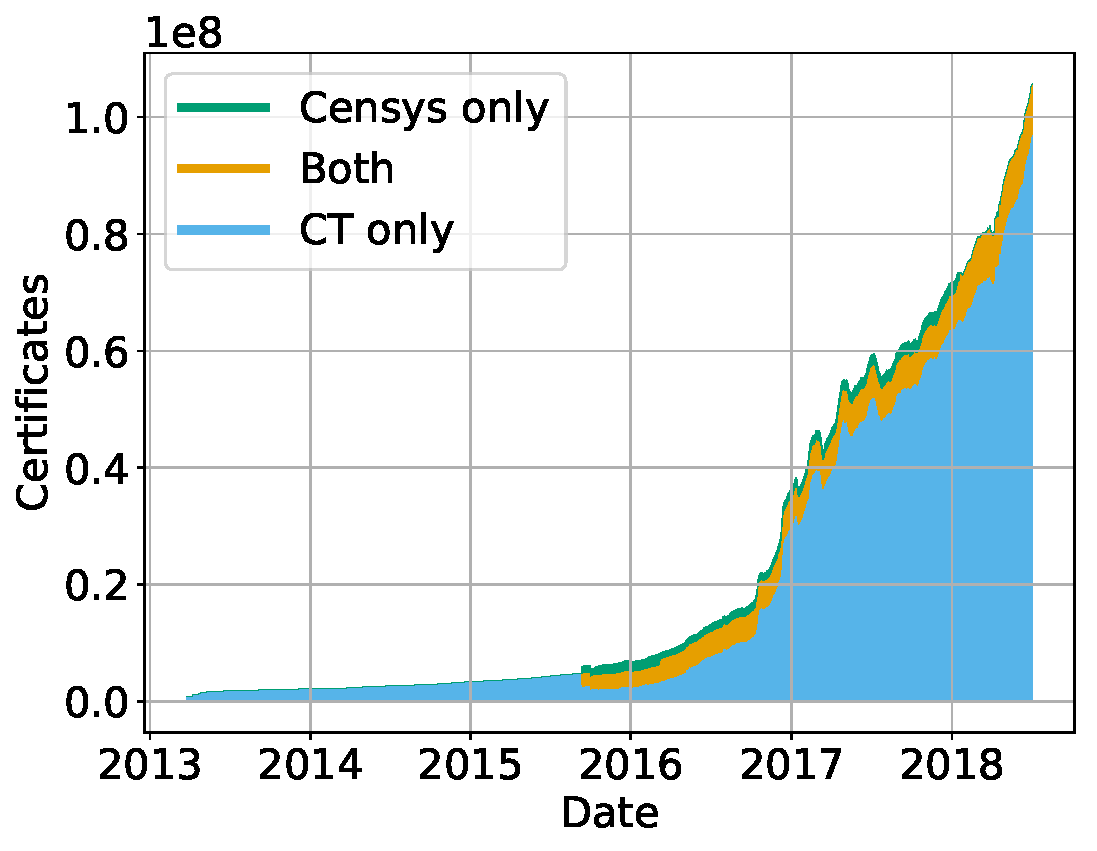
\includegraphics[width=\linewidth]{fig/cert_count_valid}
  \caption{Number of HTTPS-enabled domains over time.}
\label{fig:certs}
\end{figure}

\begin{figure}
  \centering
  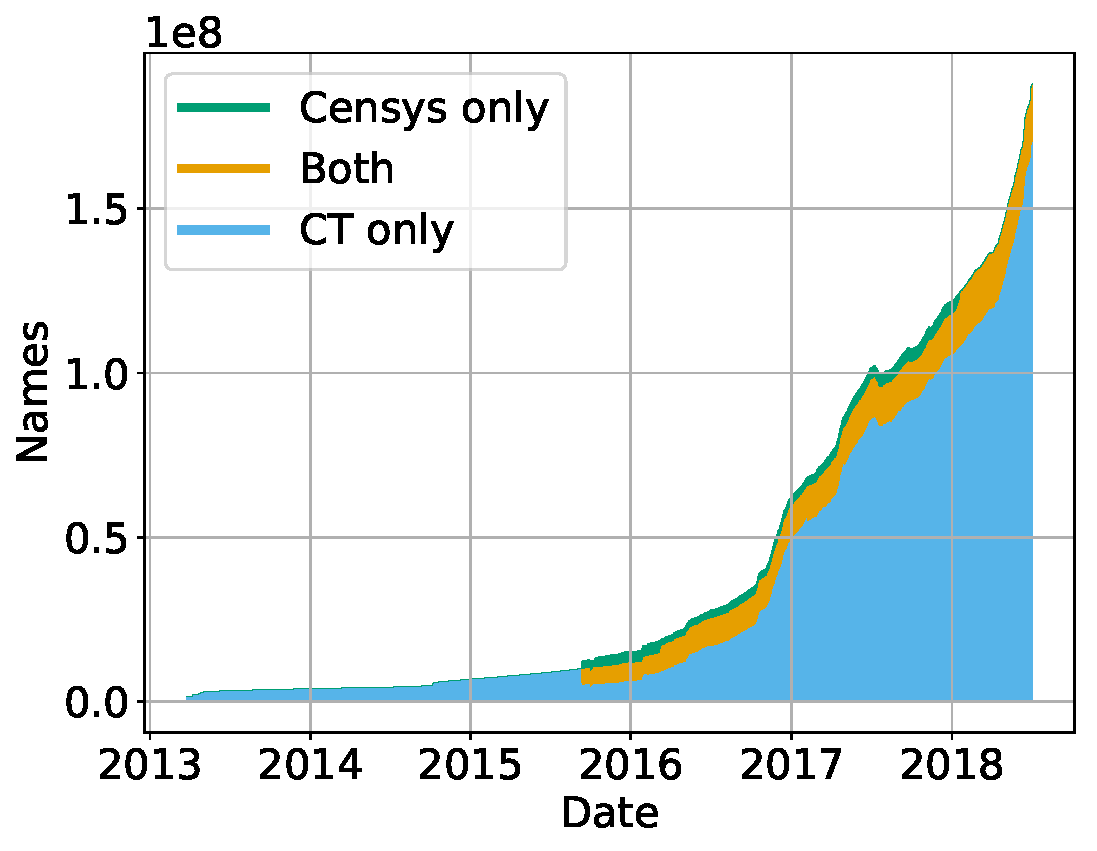
\includegraphics[width=\linewidth]{fig/name_count_valid}
  \caption{Number of HTTPS-enabled domains over time.}
  \label{fig:cert-add-exp}
\end{figure}

Because HTTPS adoption trends changed during our measurement period, we focus on
the last two years of data, from 3 July 2016 to 3 July 2018, which we show in
\autoref{fig:certs}. There are close to 200 million distinct \acp{fqdn}
currently associated with \iac{https} certificates. We did not find a clear
trend that encompassed the entire range of the data, but we observe a roughly
linear trend from April to July 2018. Specifically, the set of \acp{fqdn} that
deploy \ac{https} grows at an average of 574,921 names per day, with $R^2=0.97$.

\steve{Further things to explore:
  \begin{compactitem}
  \item How much data is captured in Censys vs \ac{ct}
  \item Scale of \acp{fqdn} in Alexa Top 1M sites
  \item List of names under the public suffix list
  \item Overall trends for \ac{fqdn} growth
  \item When names that expire reappear
  \item Issuers/domains that don't renew before expiration
  \end{compactitem}
}

\subsection{Implementation}
\label{sec:evaluation:implementation}

We prototyped the client software as a Mozilla Firefox plugin.

\begin{compactitem}
\item Update sizes
\item Memory usage
\item Disk storage size
\item Connection latency
\end{compactitem}

\steve{TODO: how much space efficiency do we lose if we separate out domains?}

\steve{TODO: also compare with set of domains covered by HTTPS Everywhere for
comparison}

\subsection{Performance}
\label{sec:evaluation:performance}

\begin{compactitem}
\item Changes to the signaling set (what domains change and overall growth)
\item Time to create/update set
\end{compactitem}

\subsection{Log Aggregator}

\begin{compactitem}
\item Size of aggregated log data over time (shows storage overhead and growth)
\item Mapping size vs. number of certificates
\end{compactitem}

%\subsection{Policy Mechanism}

%\draft{We implemented a log that tracks policies. Our code is in \steve{TODO}.
%We measured its performance and storage requirements given realistic rates of
%new certificates.}

%\subsection{Signaling Mechanism}

%We implemented our signal set construction in C++.

%\draft{We compare our approach to simple compression of the list of deploying
%domains, and to succinct encodings of a prefix tree (trie). We measure the
%compressed size, memory footprint, and added connection latency.}

%\steve{TODO: Add projections on how the metrics will change if there are $n$
%deploying domains.}

%\textbf{Failures of a Probabilistic Approach.} While at first it may seem that
%data structures implementing probabilistic membership queries (i.e., Bloom
%filters~\cite{bloom1970space} and their variants) could provide much of the
%benefits of a signaling set with only a small cost, this approach has several
%critical shortcomings. First, Bloom filters allow false positives but no false
%negatives. Therefore, while clients are protected from \ac{mitm} attacks that
%could result from false negatives, clients may be blocked from accessing sites
%that do not deploy \ac{https} because they are false positives in the Bloom
%filter. Second, on average, a Bloom filter with false positive probability
%\bloomfpp requires approximately $-\ln \bloomfpp/(\ln 2)^2$ bits per inserted
%element in the optimal case. Thus for a false positive rate of $p = 0.01$ (which
%would still cause 10,000 sites out of 1M sites deploying \ac{https} to be
%blocked), we would require 9.59 bits per site on average. Thus for our full data
%set, a Bloom filter would require \steve{145 MB}.
